%\documentclass[12pt,a4paper]{scrartcl}
\documentclass[12pt,a4paper]{article}

\makeatletter % Technical doc - START

\usepackage[utf8]{inputenc}
\usepackage[T1]{fontenc}
\usepackage{ucs}

\usepackage[french]{babel,varioref}

\usepackage[top=2cm, bottom=2cm, left=1.5cm, right=1.5cm]{geometry}
\usepackage{enumitem}

\usepackage{pgffor}

\usepackage{multicol}

\usepackage{makecell}

\usepackage{color}
\usepackage{hyperref}
\hypersetup{
    colorlinks,
    citecolor=black,
    filecolor=black,
    linkcolor=black,
    urlcolor=black
}

\usepackage{amsthm}

\usepackage{tcolorbox}
\tcbuselibrary{listingsutf8}

\usepackage{ifplatform}

\usepackage{ifthen}

\usepackage{macroenvsign}


% Sections numbering

%\renewcommand\thechapter{\Alph{chapter}.}
\renewcommand\thesection{\Roman{section}.}
\renewcommand\thesubsection{\arabic{subsection}.}
\renewcommand\thesubsubsection{\roman{subsubsection}.}



% MISC

\newtcblisting{latexex}{%
	sharp corners,%
	left=1mm, right=1mm,%
	bottom=1mm, top=1mm,%
	colupper=red!75!blue,%
	listing side text
}

\newtcbinputlisting{\inputlatexex}[2][]{%
	listing file={#2},%
	sharp corners,%
	left=1mm, right=1mm,%
	bottom=1mm, top=1mm,%
	colupper=red!75!blue,%
	listing side text
}


\newtcblisting{latexex-flat}{%
	sharp corners,%
	left=1mm, right=1mm,%
	bottom=1mm, top=1mm,%
	colupper=red!75!blue,%
}

\newtcbinputlisting{\inputlatexexflat}[2][]{%
	listing file={#2},%
	sharp corners,%
	left=1mm, right=1mm,%
	bottom=1mm, top=1mm,%
	colupper=red!75!blue,%
}


\newtcblisting{latexex-alone}{%
	sharp corners,%
	left=1mm, right=1mm,%
	bottom=1mm, top=1mm,%
	colupper=red!75!blue,%
	listing only
}

\newtcbinputlisting{\inputlatexexalone}[2][]{%
	listing file={#2},%
	sharp corners,%
	left=1mm, right=1mm,%
	bottom=1mm, top=1mm,%
	colupper=red!75!blue,%
	listing only
}


\newcommand\inputlatexexcodeafter[1]{%
	\begin{center}
		\input{#1}
	\end{center}

	\vspace{-.5em}
	
	Le rendu précédent a été obtenu via le code suivant.
	
	\inputlatexexalone{#1}
}


\newcommand\inputlatexexcodebefore[1]{%
	\inputlatexexalone{#1}
	\vspace{-.75em}
	\begin{center}
		\textit{\footnotesize Rendu du code précédent}
		
		\medskip
		
		\input{#1}
	\end{center}
}


\newcommand\env[1]{\texttt{#1}}
\newcommand\macro[1]{\env{\textbackslash{}#1}}



\setlength{\parindent}{0cm}
\setlist{noitemsep}

\theoremstyle{definition}
\newtheorem*{remark}{Remarque}

\usepackage[raggedright]{titlesec}

\titleformat{\paragraph}[hang]{\normalfont\normalsize\bfseries}{\theparagraph}{1em}{}
\titlespacing*{\paragraph}{0pt}{3.25ex plus 1ex minus .2ex}{0.5em}


\newcommand\separation{
	\medskip
	\hfill\rule{0.5\textwidth}{0.75pt}\hfill
	\medskip
}


\newcommand\extraspace{
	\vspace{0.25em}
}


\newcommand\whyprefix[2]{%
	\textbf{\prefix{#1}}-#2%
}

\newcommand\mwhyprefix[2]{%
	\texttt{#1 = #1-#2}%
}

\newcommand\prefix[1]{%
	\texttt{#1}%
}


\newcommand\inenglish{\@ifstar{\@inenglish@star}{\@inenglish@no@star}}

\newcommand\@inenglish@star[1]{%
	\emph{\og #1 \fg}%
}

\newcommand\@inenglish@no@star[1]{%
	\@inenglish@star{#1} en anglais%
}


\newcommand\ascii{\texttt{ASCII}}


% Example
\newcounter{paraexample}[subsubsection]

\newcommand\@newexample@abstract[2]{%
	\paragraph{%
		#1%
		\if\relax\detokenize{#2}\relax\else {} -- #2\fi%
	}%
}



\newcommand\newparaexample{\@ifstar{\@newparaexample@star}{\@newparaexample@no@star}}

\newcommand\@newparaexample@no@star[1]{%
	\refstepcounter{paraexample}%
	\@newexample@abstract{Exemple \theparaexample}{#1}%
}

\newcommand\@newparaexample@star[1]{%
	\@newexample@abstract{Exemple}{#1}%
}


% Change log
\newcommand\topic{\@ifstar{\@topic@star}{\@topic@no@star}}

\newcommand\@topic@no@star[1]{%
	\textbf{\textsc{#1}.}%
}

\newcommand\@topic@star[1]{%
	\textbf{\textsc{#1} :}%
}

\makeatother % Technical doc - END


\usepackage{tnslog}


\begin{document}

\renewcommand\labelitemi{\raisebox{0.125em}{\tiny\textbullet}}
\renewcommand{\labelitemii}{---}

\title{  %
	Le package \texttt{tnslog}:\\%
	rédiger de la logique simple\\%
	{\footnotesize Code source disponible sur \url{https://github.com/typensee-latex/tnslog.git}.}\\%
{\footnotesize Version \texttt{0.0.0-beta} développée et testée sur \macosxname{}.}%
}
\author{Christophe BAL}
\date{2020-07-10}

\maketitle


\vspace{2em}

\hrule

\tableofcontents

\vspace{1.5em}

\hrule

\newpage

\section{Introduction}

Le package \verb+tnslog+ facilite la rédaction de preuves formelles basiques via un codage sémantique simple.


% tnscom used - START
\section{Beta-dépendance}

\verb#tnscom# qui est disponible sur \url{https://github.com/typensee-latex/tnscom.git} est un package utilisé en coulisse.
% tnscom used - END
% List of packages - START
\section{Packages utilisés}

La roue ayant déjà été inventée, le package \verb#tnslog# réutilise les packages suivants sans aucun scrupule.

\begin{multicols}{4}
    \begin{itemize}
        \item \verb#amssymb#
        \item \verb#centernot#
        \item \verb#etoolbox#
        \item \verb#longtable#
        \item \verb#mathtools#
        \item \verb#simplekv#
        \item \verb#witharrows#
    \end{itemize}
\end{multicols}
% List of packages - END
%\section{Quelques modifications générales}

\section{Espace après la négation logique}

\macro{neg} a été redéfinie pour ajouter un peu d'espace après le symbole. Le comportement par défaut se retrouve en utilisant la macro \macro{stdneg}. Voici un exemple.


\begin{latexex}
$\neg A = \stdneg A$

$\neg\neg A = \stdneg \stdneg A$
\end{latexex}


% ---------------------- %
\section{Différents types de comparaisons \og standard \fg}

D'un point de vue pédagogique, il peut être intéressant de disposer de différentes façon d'écrire une égalité, une non égalité ou une inégalité.
Bien entendu on tord les règles de typographie avec ce type de pratique mais c'est pour le bien de la communauté éducative.


\subsection{Définir quelque chose}

L'exemple suivant montre deux façons de rédiger une égalité signifiant une définition \emph{(la section \ref{tnslog-texts-for-opes} explique comment est défini le texte \emph{\og \textopdef \fg})}.

\begin{latexex}
$f(x) \eqdef x^3 + 1$

$f(x) \eqdef* x^3 + 1$
\end{latexex}


% ---------------------- %


\subsection{Indiquer une identité}

L'exemple suivant montre deux façons de rédiger des identités avec une notation symbolique non standard \emph{(la section \ref{tnslog-texts-for-opes} explique comment est défini le texte \emph{\og \textopid \fg})}.

\begin{latexex}
$(a + b)^2 \eqid a^2 + b^2 + 2 a b$

$(a + b)^2 \eqid* a^2 + b^2 + 2 a b$
\end{latexex}


% ---------------------- %


\subsection{Une égalité à vérifier ou non, une hypothèse, une condition}

Se reporter à la section \ref{tnslog-texts-for-opes} pour savoir comment sont définis les textes \emph{\og \textopcons \fg} , \emph{\og \textopcond \fg} et \emph{\og \textophyp \fg}.

\begin{latexex}
$(a + b)^3 \eqtest a^3 + b^3 + 3 a b$

$(a + b)^3 \neqid a^3 + b^3 + 3 a b$

$x \neqhyp 0$  ou
$x \neqcond 0$ ou
$x \eqcons 0$
\end{latexex}


% ---------------------- %


\subsection{Une égalité indiquant le choix d'une valeur ou l'application d'une relation}

La section \ref{tnslog-texts-for-opes} permet de savoir comment les textes \emph{\og \textopchoice \fg} et \emph{\og \textopappli \fg} sont définis.

\begin{latexex}
$x \geqcond 4$ implique
$x^2 \geqcons 16$.

Donc $x \eqchoice 123$ donne
$123^2 \geqappli 16$.
\end{latexex}


% ---------------------- %


\subsection{Une égalité indiquant l'équation d'une courbe}

La section \ref{tnslog-texts-for-opes} permet de savoir comment les texte \emph{\og \textopplot \fg} est défini.

\begin{latexex}
$M \in C: y \eqplot x^2 + 3$
donne
$y_M \eqappli x_M^2 + 3$.
\end{latexex}


% ---------------------- %


\subsection{Différents types d'inéquations}

Le principe reste le même pour les symboles d'équations excepté qu'il n'y a ici aucune écriture purement symbolique. Voici un code \og fourre-tout \fg{} montrant quelques exemples.

\begin{latexex}
$x \leqtest x^2$ ou $x \lesscons x^2$ ou
$x \geqhyp 1$    ou $x \gtrcond 2$.
\end{latexex}


% ---------------------- %


\subsection{Des formes négatives aussi pour les inéquations}

Tous les opérateurs de comparaison ont une forme négative qui s'obtient en préfixant le nom de l'opérateur par \verb+n+.
Voici quelques exemples d'utilisation.

\begin{latexex}
$x \nlesshyp 3$ ou
$y \nleqtest 4$ ou
$z \ngeqcons 5$
\end{latexex}


% ---------------------- %


\subsection{Une table récapitulative}

La table \ref{tnslog-table:deco-opes} \vpageref{tnslog-table:deco-opes} fournit toutes les associations autorisées entre opérateurs de comparaison et décorations.


% ---------------------- %


\subsection{Textes utilisés} \label{tnslog-texts-for-opes}

Voici les macros définissant les textes utilisés qui tiennent compte de l'utilisation ou non de l'option \verb+french+ de \verb+babel+. Nous ne donnons que les versions françaises.

\vspace{-.5em}

\begin{center}
	\begin{tabular}{l@{\kern1ex}l@{\kern2cm}l@{\kern1ex}l}
% == All texts - START == %
        \macro{textopappli\{\}} & donne \emph{\og \textopappli \fg}
        & \macro{textopchoice\{\}} & donne \emph{\og \textopchoice \fg} \\
        \macro{textopcond\{\}} & donne \emph{\og \textopcond \fg}
        & \macro{textopcons\{\}} & donne \emph{\og \textopcons \fg} \\
        \macro{textopdef\{\}} & donne \emph{\og \textopdef \fg}
        & \macro{textophyp\{\}} & donne \emph{\og \textophyp \fg} \\
        \macro{textopid\{\}} & donne \emph{\og \textopid \fg}
        & \macro{textopplot\{\}} & donne \emph{\og \textopplot \fg} \\
        \macro{textoptest\{\}} & donne \emph{\og \textoptest \fg}
        & & \\
% == All texts - END == %
	\end{tabular}
\end{center}

% ---------------------- %
\section{Équivalences et implications}

\subsection{Des symboles logiques supplémentaires}

\newparaexample{Implication réciproque}

En plus des opérateurs \macro{iff} et \macro{implies} proposés par \LaTeX{}, il a été ajouté l'opérateur \macro{liesimp}, où l'on a inversé les groupes syllabiques de \macro{implies}, un opérateur pour pour obtenir $\liesimp$
\footnote{
	Penser aussi aux preuves d'équivalence par double implication.
},
ainsi que des versions négatives. Voici un exemple d'utilisation.

\begin{latexex}
$(A \implies B)
 \iff (B \liesimp A)$

$(A \implies B)
 \niff (A \nimplies B)$
\end{latexex}


% ---------------------- %


\newparaexample{Des opérateurs décorés}

Tout comme pour les comparaisons, il existe des versions décorées de type test, hypothèse, condition \dots{} 
Elles sont toutes présentes dans l'exemple suivant.

\begin{latexex}
$A \iffappli B \niffchoice C$

$A \impliescond B \nimpliescons C$

$A \liesimphyp B \nliesimptest C$
\end{latexex}


% ---------------------- %


\subsection{Une table récapitulative}

La table \ref{tnslog-table:deco-opes} \vpageref{tnslog-table:deco-opes} montre toutes les associations autorisées entre opérateurs logiques et décorations.


% ---------------------- %


\subsection{Équivalences et implications verticales}

\paragraph{À quoi cela sert-il ?}

Les sections \ref{tnslog-explain-proof} et \ref{tnslog-explain-proof-for-youngs} présentent deux environnements pour détailler les étapes d'un raisonnement.
Avec ces outils il devient utile d'avoir des versions verticales non décorées des symboles d'équivalence et d'implication. Voici comment les obtenir \emph{(tous les cas possibles ont été indiqués)}.
Bien entendu le préfixe \prefix{v} est pour \whyprefix{v}{ertical}.

\begin{latexex}
\begin{tabular}{cccccc}
    $A$          & $B$
  & $C$          & $D$
  & $E$          & $F$
  \\
    $\viff$      & $\vimplies$   
  & $\vliesimp$  & $\nviff$
  & $\nvimplies$ & $\nvliesimp$
  \\
    $A$          & $B$
  & $C$          & $D$
  & $E$          & $F$
\end{tabular}
\end{latexex}


% ---------------------- %
%\section{Logique et fondements}

\subsection{Tables des décorations possibles des opérateurs}

La table \ref{tnslog-table:deco-opes} \vpageref{tnslog-table:deco-opes} donne toutes les associations autorisées entre opérateurs et décorations.
Il faut retenir que les versions étoilées produisent des écritures symboliques. 


% == Table - START == %

\begin{table}[h]
    \caption{Décorations}
    \begin{center}
        \begin{tabular}{c|c|c|c|c|c|c|c|c|c|c|c}
             Préfixe & \verb+appli+ & \verb+choice+ & \verb+cond+ & \verb+cons+ & \verb+def+ & \verb+def*+ & \verb+hyp+ & \verb+id+ & \verb+id*+ & \verb+plot+ & \verb+test+ \\
            \hline \makecell{\macro{eq}} & $\times$ & $\times$ & $\times$ & $\times$ & $\times$ & $\times$ & $\times$ & $\times$ & $\times$ & $\times$ & $\times$ \\
            \hline \makecell{\macro{neq}} & $\times$ & $\times$ & $\times$ & $\times$ &          &          & $\times$ & $\times$ &          & $\times$ & $\times$ \\
            \hline \makecell{\macro{less}\\\macro{nless}\\\macro{leq}\\\macro{nleq}\\\macro{gtr}\\\macro{ngtr}\\\macro{geq}\\\macro{ngeq}} & $\times$ & $\times$ & $\times$ & $\times$ &          &          & $\times$ &          &          & $\times$ & $\times$ \\
            \hline \makecell{\macro{iff}\\\macro{niff}\\\macro{implies}\\\macro{nimplies}\\\macro{liesimp}\\\macro{nliesimp}} & $\times$ & $\times$ & $\times$ & $\times$ &          &          & $\times$ &          &          &          & $\times$ \\
        \end{tabular}
    \end{center}
    \label{tnslog-table:deco-opes}
\end{table}

% == Table - END == %
\section{Des versions alternatives du quantificateur existentiel}

\subsection{Quantifier l'existence}

Voici deux versions, l'une classique, et l'autre beaucoup moins, permettant de préciser le quantificateur $\exists$.

\begin{latexex}
$\existsone x \in E$ pour
\og il existe un seul $x$ \fg.

$\existmulti{\leq 1} y \in F$ pour
\og il existe au plus un $y$ \fg.

$\existmulti{=1} \eqdef* \existsone$
\end{latexex}


% ---------------------- %


\subsection{Versions négatives}

\begin{latexex}
$\nexistsone$ pour
\og il n'existe pas un unique \fg.

$\existmulti{\neq1} \eqdef* \nexistsone$

$\nexistmulti{>4}$ pour
\og il n'existe pas plus de quatre \fg.

$\nexists$ vient de \verb+amssymb+.
\end{latexex}


% ---------------------- %
\section{Détailler un raisonnement simple}

\subsection{Version pour le lycée et après} \label{tnslog-explain-proof}

\newparaexample{Avec les réglages par défaut}

L'environnement \env{explain} permet de détailler les étapes principales d'un calcul ou d'un raisonnement simple en s'appuyant sur la macro \macro{explnext} dont le nom vient de \emph{\og \whyprefix{expl}{ain} \prefix{next} step \fg} soit \inenglish{expliquer la prochaine étape}
\footnote{
    Cet environnement utilise aussi le package \texttt{witharrows} qui est très sympathique pour expliquer des étapes de calcul.
}.
On dispose aussi de \macro{explnext*} pour des explications descendantes et/ou montantes 
\footnote{
    Les explications données ne doivent pas être trop longues car ce serait contre-productif.
}.

\medskip


Ci-dessous se trouve un exemple, très farfelu vers la fin, où l'on utilise les réglages par défaut.
Notons au passage que ce type de présentation n'est sûrement pas bien adaptée à un jeune public pour lequel une 2\ieme{} façon de détailler des calculs et/ou un raisonnement simple est proposée plus bas dans la section \ref{tnslog-explain-proof-for-youngs}.

\begin{latexex-flat}
\begin{explain}
    (a + b)^2
        \explnext{On utilise $x^2 = x \cdot x$.}
    (a + b) (a + b)
        \explnext*{Double développement depuis la parenthèse gauche.}%
                  {Double factorisation pas facile.}
    a^2 + a b + b a + b^2
        \explnext*{}%
                  {Commutativité du produit.}
    a^2 + 2 a b + b^2
        \explnext*{Commutativité de l'addition.}%
                  {}
    a^2 + b^2 + 2 a b
\end{explain}
\end{latexex-flat}


\begin{remark}
    Il faut savoir que la mise en forme est celle d'une formule ce qui peut rendre service comme dans l'exemple suivant.

\begin{latexex}
Un calcul avec un placement pouvant être 
utile :
\begin{explain}
    (a + b)^2
        \explnext{Identité remarquable.}
    a^2 + b^2 + 2 a b
\end{explain}
\end{latexex}

Avec un retour à la ligne, il faudra donc si besoin gérer l'espacement vertical.

\begin{latexex}
Mon calcul pas trop proche.

\medskip
\begin{explain}
    (a + b)^2
        \explnext{Identité remarquable.}
    a^2 + b^2 + 2 a b
\end{explain}
\end{latexex}
\end{remark}


\begin{remark}
    Voici des petites choses à connaître sur les macros \macro{explnext} et \macro{explnext*}.
    \begin{enumerate}
        \item \macro{expltxt} est utilisée par \macro{explnext} pour mettre en forme le texte d'explication.

        \item \macro{expltxtup} et \macro{expltxtdown} sont utilisées par \macro{explnext*} décorer les textes d'explication juste avant leur mise en forme finale via \macro{expltxtupdown}.

        \item \macro{explnext} et \macro{explnext*} utilisent la macro constante \macro{expltxtspacein} pour l'espacement entre le symbole et la courte explication. Par défaut, cette macro vaut \verb+2em+.
    \end{enumerate}
 
\end{remark}


% ---------------------- %


\newparaexample{Utiliser un autre symbole globalement}

L'environnement \env{explain} possède plusieurs options dont l'une est \verb+ope+ qui vaut \verb+{=}+ par défaut. Ceci permet de faire ce qui suit sans effort.

\begin{latexex}
\begin{explain}[ope = \viff]
    x^2 + 10 x + 25 = 0
        \explnext{Identité remarquable.}
    (x + 5)^2 = 0
        \explnext{$P^2 = 0$ si et 
                  seulement si $P = 0$.}
    x = -5
\end{explain}
\end{latexex}


% ---------------------- %


\newparaexample{Juste utiliser des symboles}

Si l'argument obligatoire de la macro \macro{explnext} est vide alors seul le symbole est affiché \emph{(ne pas oublier les accolades vides)}. Voici un court exemple de ceci.

\begin{latexex}
\begin{explain}[ope = \viff]
    a^2 = b^2
        \explnext{}
    a = \pm b
\end{explain}
\end{latexex}


% ---------------------- %


\newparaexample{Utiliser un autre symbole localement}

La macro \macro{explnext} possède un argument optionnel qui utilise par défaut celui de l'environment. En utilisant cette option, on choisit alors localement le symbole à employer. Voici un exemple d'utilisation complètement farfelu bien que correct.

\begin{latexex}
\begin{explain}[ope = \viff]
    0 \leq a < b
        \explnext[\vimplies]%
                 {Croissance de $x^2$ 
                  sur $R_{+}$.}
    a^2 < b^2
        \explnext{}
    a^2 - b^2 < 0
        \explnext{Identité remarquable.}
    (a - b)(a + b) < 0
        \explnext[\vimplies]{}
    a \neq b
\end{explain}
\end{latexex}


% ---------------------- %


\newparaexample{Choisir la mise en forme des explications}

Pour la mise en forme des explications à double sens, la macro \macro{explnext} fait appel à la macro \macro{expltxt}.
Par défaut, le package utilise la définition suivante.

\begin{latexex-alone}
\newcommand\expltxt[1]{%
    \text{\color{blue}\footnotesize \{\,{\itshape #1}\,\} }%
}
\end{latexex-alone}


Pour la mise en forme des explications à sens unique, la macro \macro{explnext*} fait appel aux macros \macro{expltxtup}, \macro{expltxtdown} et \macro{expltxtupdown}.
Par défaut le package utilise les définitions suivantes.

\begin{latexex-alone}
\newcommand\expltxtup[1]{%
    $\uparrow$ #1 $\uparrow$%
}

\newcommand\expltxtdown[1]{%
    $\downarrow$ #1 $\downarrow$%
}

\newcommand\expltxtupdown[2]{{%
    \displaystyle\footnotesize\color{blue}%
    \left\{\,%
        \genfrac{}{}{0pt}{}{%
            \text{\itshape\expltxtdown{\samesizeas{#1}{#2}}}%
        }{%
            \text{\itshape\expltxtup{\samesizeas{#2}{#1}}}%
        }%
    \,\right\}%
}}
\end{latexex-alone}


Nous allons expliquer comment obtenir l'affreux exemple ci-dessous montrant que l'on peut adapter si besoin la mise en forme.

% ==================== %

\bgroup

\newcommand\myexpltxt[2]{%
    \text{\color{#1} \footnotesize \itshape \bfseries #2}%
}

\renewcommand\expltxt[1]{%
    \myexpltxt{gray}{$\Downarrow$ #1 $\Uparrow$}%
}

\renewcommand\expltxtup[1]{%
    \myexpltxt{orange}{$\Uparrow$ #1 $\Uparrow$}%
}

\renewcommand\expltxtdown[1]{%
    \myexpltxt{red}{$\Downarrow$ #1 $\Downarrow$}%
}

\renewcommand\expltxtupdown[2]{%
    \displaystyle\color{blue!20!black!30!green}\genfrac{\langle}{\rangle}{1pt}{}{%
        \expltxtdown{\samesizeas{#1}{#2}}%
    }{%
        \expltxtup{\samesizeas{#2}{#1}}%
    }%
}


\begin{latexex}
\begin{explain}
    (a + b) (a + b)
        \explnext{Se souvenir de $P\cdot P = P^2$.}%
    (a + b)^2
        \explnext*{Id. Rm. - Dév.}%
                  {Id. Rm. - Facto.}
    a^2 + 2 a b + b^2
\end{explain}
\end{latexex}

\egroup


La mise en forme a été obtenue en utilisant le code \LaTeX{} suivant où la macro \macro{samesizeas\{\#1\}\{\#2\}} rend le texte \verb+#1+ aussi large que \verb+#2+ en ajoutant des espaces supplémentaires tout en centrant le résultat final si besoin  \emph{(ne pas oublier de passer en mode texte via \macro{text})}.

\begin{latexex-alone}
\newcommand\myexpltxt[2]{%
    \text{\color{#1} \footnotesize \itshape \bfseries #2}%
}

\renewcommand\expltxt[1]{%
    \myexpltxt{gray}{$\Downarrow$ #1 $\Uparrow$}%
}

\renewcommand\expltxtup[1]{%
    \myexpltxt{orange}{$\Uparrow$ #1 $\Uparrow$}%
}

\renewcommand\expltxtdown[1]{%
    \myexpltxt{red}{$\Downarrow$ #1 $\Downarrow$}%
}

\renewcommand\expltxtupdown[2]{%
    \displaystyle\color{blue!20!black!30!green}%
    \genfrac{\langle}{\rangle}{1pt}{}{%
        \expltxtdown{\samesizeas{#1}{#2}}%
    }{%
        \expltxtup{\samesizeas{#2}{#1}}%
    }%
}
\end{latexex-alone}


% ==================== %
%\section{Détailler un raisonnement simple}

\subsection{Version pour les collégiens} \label{tnslog-explain-proof-for-youngs}

L'environnement \env{explain} avec l'option \verb+style = ar+
\footnote{
    Cet environnement utilise aussi le package \texttt{witharrows}.
}
utilise des flèches pour indiquer les explications
\emph{(\prefix{ar} est pour \whyprefix{ar}{row} soit \inenglish{flèche})}.
Dans ce cas d'utilisation, la macro \macro{explnext*} permet d'avoir une flèche unidirectionnelle, vers le haut ou le bas au choix, ou bien d'écrire deux indications dont l'une est montante et l'autre descendante.

\medskip

Il existe aussi l'option \verb+style = sar+ lorsque la toute 1\iere{} étape n'est pas expliquée
\emph{(\prefix{s} est pour \whyprefix{s}{hort} soit \inenglish{court})}.
Attention car forcément ceci nécessite au tout début de l'environnement l'usage de la macro \macro{explnext} sans aucun contenu !


% ---------------------- %


\newparaexample{Des flèches à double sens}

\begin{latexex}
\begin{explain}[style = ar]
    (a + b)^2
        \explnext{Identité remarquable}
    a^2 + 2 a b + b^2
        \explnext{}
    a^2 + b^2 + 2 a b
\end{explain}
\end{latexex}


% ---------------------- %


\newparaexample{Des flèches unidirectionnelles}

Ce qui suit est juste là comme démo. car les explications y sont un peu farfelues.

\begin{latexex-flat}
\begin{explain}[style = ar]
    (a + b)^2
        \explnext*{Via $P^2 = P \cdot P$.}
                  {Via $P \cdot P = P^2$.}
    (a + b) (a + b)
        \explnext*{Double développement.}%
                  {Double factorisation (pas simple).}
    a^2 + a b + b a + b^2
        \explnext*{Commutativité du produit.}%
                  {}
    a^2 + 2 a b + b^2
        \explnext*{}%
                  {Commutativité de l'addition.}
    a^2 + b^2 + 2 a b
\end{explain}
\end{latexex-flat}


% ---------------------- %


\newparaexample{Ne pas expliquer le tout début}

L'environnement étoilé \env{explain} avec l'option \verb+style = sar+ débute différemment la mise en forme.
Bien entendu ici le tout premier \macro{explnext} doit avoir un argument vide !

\begin{latexex-flat}
\begin{explain}[style = sar]
    (a + b) (a + b)
        \explnext{}
    (a + b)^2
        \explnext{Identité remarquable.}
    a^2 + b^2 + 2 a b
\end{explain}
\end{latexex-flat}


% ---------------------- %


\newparaexample{Choisir son symbole}

Voici comment faire où l'implication finale est juste là pour la démonstration \emph{(on notera une petite bidouille un peu sale à faire pour avoir un alignement à peu près correct)}.

\begin{latexex}
\begin{explain}[style = ar, ope = \iff]
    a^2 + 2 a b + b^2 = 0
        \explnext{}
    (a + b)^2 = 0
        \explnext[\:\implies]%
                 {$P^2 = 0$ ssi $P = 0$.}
    a + b = 0
\end{explain}
\end{latexex}


Avec la version courte, on obtient ce qui suit.

\begin{latexex-flat}
\begin{explain}[style = sar, ope = \iff]
    a^2 + 2 a b + b^2 = 0
        \explnext{}
    (a + b)^2 = 0
        \explnext[\:\implies]%
                 {$P^2 = 0$ ssi $P = 0$.}
    a + b = 0
\end{explain}
\end{latexex-flat}
%\section{Détailler un raisonnement simple}

\subsection{De courts commentaires}

\newparaexample{Sans alignement}

Il est possible d'ajouter de petits commentaires via \macro{comthis} où \prefix{comthis} est pour \whyprefix{com}{ment} \prefix{this} soit \inenglish{commenter ceci}.
 
\begin{latexex}
\begin{explain}
    (a + b)^2
        \comthis{Forme facto.}
        \explnext*{Id.Rq. -- Dév.}%
                  {Id.Rq. -- Facto.}
    a^2 + 2 a b + b^2
        \comthis{Forme dév.}
\end{explain}
\end{latexex}


\begin{remark}
	La mise en forme du texte des commentaires est fait via la macro personnalisable \macro{explcom}.
	Quant à l'espacement ajouté entre le texte et son commentaire il est défini par la macro \macro{expltxtspacein} qui est égale à \verb+2em+ par défaut.
\end{remark}


% ---------------------- %


\newparaexample{Tout aligner}

Il peut être utile d'aligner tous les commentaires. Ceci s'obtient via l'option \verb+com = al+ où \prefix{al} est pour \whyprefix{al}{igné} \emph{(par défaut \prefix{com = nal} avec le préfixe \prefix{n} pour \whyprefix{n}{on})}.

\begin{latexex}
\begin{explain}[com = al]
    (a + b)^2
        \comthis{Forme facto.}
        \explnext*{Id.Rq - Dév.}%
                  {Id.Rq - Facto.}
    a^2 + 2 a b + b^2
        \comthis{Forme dév.}
\end{explain}
\end{latexex}


% ---------------------- %


\newparaexample{Le meilleur des deux mondes}

Dans d'autres situations, utilisez les deux types d'alignement peut faire sens. Ceci s'obtient via l'option \verb+com = al+ et l'emploi de la macro étoilée \macro{comthis*} à chaque fois que l'on souhaite "coller" un commentaire le plus à gauche possible.

\begin{latexex}
\begin{explain}[com = al]
    (a + b) (a + b)
        \comthis{Forme facto.}
        \explnext{Via $x^2 = x \cdot x$.}
    (a + b)^2
        \comthis*{Au passage...}
        \explnext*{Id.Rq - Dév.}%
                  {Id.Rq - Facto.}
    a^2 + 2 a b + b^2
        \comthis{Forme dév.}
\end{explain}
\end{latexex}


\begin{remark}
	Si l'alignement n'est pas activé, les macros \macro{comthis*} et \macro{comthis} auront toutes les deux le même effet.
\end{remark}


% ---------------------- %


\newparaexample{Ceci marche aussi avec le style \og fléché \fg}

Voici ce que donne le mode mixte lorsque des flèches sont utilisées pour les explications. Il semble moins pertinent ici de mixer les modes \og alignement \fg{} et \og non alignement \fg{} mais chacun pris séparément peut avoir son utilité.

\begin{latexex-flat}
\begin{explain}[style = ar, com = al]
    (a + b) (a + b)
        \comthis{Forme facto.}
        \explnext{Via $x^2 = x \cdot x$.}
    (a + b)^2
        \comthis*{Au passage...}
        \explnext*{Id.Rq - Dév.}%
                  {Id.Rq - Facto.}
    a^2 + 2 a b + b^2
        \comthis{Forme dév.}
\end{explain}
\end{latexex-flat}


\begin{remark}
	Bien entendu il est impossible de commenter le tout début en mode fléché court.
\end{remark}
%\section{Détailler un raisonnement simple}

\subsection{Un mini hack très utile pour des \emph{\og étapes alignées \fg}}

Vous pouvez écrire très facilement des calculs ou raisonnement simples alignés comme suit sans trop vous fatiguez.

\begin{latexex}
\begin{explain}[style = sar]
    (a + b) (a + b)
        \explnext{}
    (a + b)^2
        \explnext{}
    a^2 + b^2 + 2 a b
        \comthis{Pourquoi ?}
        \explnext{}
    a^2 + 2 a b + b^2
\end{explain}
\end{latexex}

On a accès à une autre mise en forme \emph{(ceci peut rendre aussi service)}. 

\begin{latexex}
\begin{explain}[style = ar]
    (a + b) (a + b)
        \explnext{}
    (a + b)^2
        \explnext{Pourquoi ?}
    a^2 + b^2 + 2 a b
        \explnext{}
    a^2 + 2 a b + b^2
\end{explain}
\end{latexex}

Enfin dans le cadre de calculs à faire expliquer par des élèves, ce qui suit peut être utile.

\begin{latexex}
Donner les justifications J1, J2 et J3.

\medskip
\begin{explain}
    (a + b) (a + b)
        \explnext{J1}
    (a + b)^2
        \explnext{J2}
    a^2 + b^2 + 2 a b
        \explnext{J3}
    a^2 + 2 a b + b^2
\end{explain}
\end{latexex}


% ---------------------- %


\subsection{Un conseil de mise en forme}

Voici un style de codage que nous trouvons très facile à relire et maintenir.

\begin{latexex}
\begin{explain}[com = al]
    (a + b) (a + b)
    	\comthis{Forme facto.}
    	\explnext{Via $x^2 = x \cdot x$.}
    %
    (a + b)^2
    	\comthis*{Au passage...}
    	\explnext*{Id.Rq - Dév.}%
                  {Id.Rq - Facto.}
    %
    a^2 + 2 a b + b^2
    	\comthis{Forme dév.}
\end{explain}
\end{latexex}
%\section{Logique et fondements}
\section{Détailler un \og vrai \fg{} raisonnement}

\subsection{Un tableau pour le post-bac}

\newparaexample{Le minimum avec les réglages par défaut}

Prenons un exemple utile à la logique formelle en informatique théorique mais qui a complètement sa place en mathématiques plus classiques \emph{(voir la section \ref{tnslog-explain-hard-proof-for-youngs} pour un autre type de présentation plus adapté à un public de collège ou de lycée)}.
Ci-dessous l'environnement \env{demoexplain} facilite la mise en page
\footnote{
	En coulisse est utilisé l'environnement \env{longtable} du package éponyme.
}
et la macro étoilée \macro{explref*} permet d'indiquer une référence interne au raisonnement
\footnote{
    Les indications peuvent être numérotes jusqu'à $99$ ce qui est bien au-delà des besoins pratiques.
}.
Dans cet exemple en deux morceaux, pour montrer au passage comment continuer la numérotation là où elle s'était arrêtée, on utilise \emph{\og m.p. \fg} comme abréviation de \emph{\og modus ponens \fg}.

\begin{latexex}
\begin{demoexplain}
    \demostep
        Hypothèse & $A$     
    \demostep
        Axiome 1  & $A \implies B$
    \demostep
        m.p. sur
        \explref*{1} et \explref*{2}
      & $B$
    \demostep
        \explref*{1} et \explref*{3}
      & $A \wedge B$
\end{demoexplain}
\end{latexex}


Il est possible de couper sa démonstration en morceaux en indiquant à l'environnement la valeur du 1\ier{} numéro de justification via la clé \verb+start+ : la valeur spéciale \verb+last+ indique de continuer la numérotation à la suite.

\begin{latexex}
\begin{demoexplain}[start = last]
    \demostep
        Axiome 3
      & $(A \wedge B) \implies C$
    \demostep
        m.p. sur
        \explref*{4} et \explref*{5}
      & $C$
\end{demoexplain}
\end{latexex}


% ---------------------- %


\newparaexample{Référencer une indication}

L'argument optionnel de \macro{demostep} permet de définir un label qui ensuite facilitera le référencement d'une justification de façon pérenne via la macro non étoilée \macro{explref}.

\begin{latexex}
\begin{demoexplain}
    \demostep[demo-my-hyp]
        Hypothèse & $A$     
    \demostep[demo-use-axiom-1]
        Axiome 1  & $A \implies B$
    \demostep
        m.p. sur
        \explref{demo-my-hyp}
        et
        \explref{demo-use-axiom-1}
      & $B$
\end{demoexplain}
\end{latexex}


\begin{remark}
    Prendre bien garde au fait que ce mécanisme utilise les macros \macro{label} et \macro{ref} de \LaTeX.
    On travaille donc avec des références globalement au document compilé.
\end{remark}


% ---------------------- %


\newparaexample{Indiquer ce que l'on cherche à faire}

Les clés optionnelles \verb+hyps+ pour plusieurs hypothèses, \verb+hyp+ pour une seule hypothèse et \verb+ccl+ pour la conclusion permettent d'expliquer ce que l'on démontre et sous quel contexte.

\begin{latexex}
\begin{demoexplain}[hyp = $A$, ccl = $B$]
    \demostep
        Hypothèse & $A$     
    \demostep
        Axiome 1  & $A \implies B$
    \demostep
        m.p. sur
        \explref*{1} et \explref*{2}
      & $B$
\end{demoexplain}
\end{latexex}


\begin{remark}
    Aucune des clés \verb+hyps+, \verb+hyp+ et \verb+ccl+ n'est obligatoire.
    Par contre il n'est pas possible d'utiliser à la fois les clés \verb+hyps+ et \verb+hyp+.
\end{remark}


% ---------------------- %


\subsection{Un tableau sur plusieurs pages}

Un tableau devant utiliser plusieurs pages sera scindé comme ci-dessous sans perte d'information
\footnote{
	Tout le travail est fait par l'environnement \env{longtable} du package éponyme.
}.

\begin{center}
	\frame{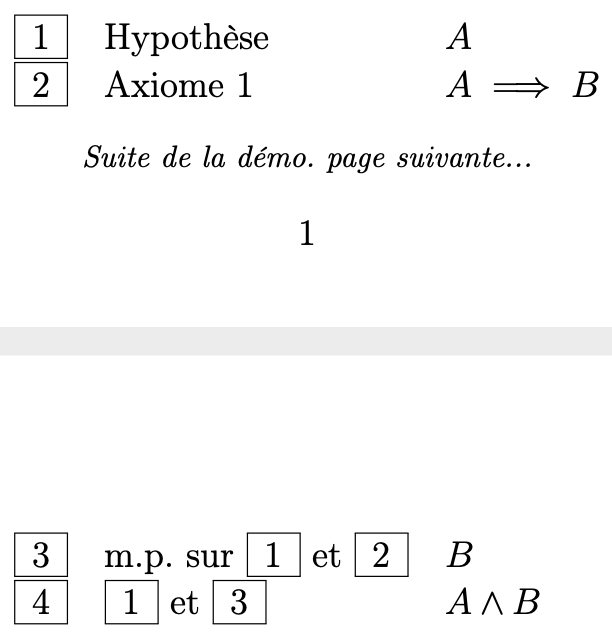
\includegraphics[scale = .5]{images/demo-explained-univ-broken[fr].png}}
\end{center}
%\section{Détailler un \og vrai \fg{} raisonnement}

\subsection{Un tableau pour le collège et le lycée} \label{tnslog-explain-hard-proof-for-youngs}


\newparaexample{Avec les réglages par défaut}

L'environnement étoilé \env{demoexplain*} est différent de l'environnement \env{demoexplain} puisqu'il sert à indiquer trois choses et non juste deux comme le montre l'exemple suivant
\footnote{
	C'est pour cela qu'est proposé une version étoilée de l'environnement et non l'utilisation d'une option de l'environnement non étoilé. 
}.
Par contre, la syntaxe est très similaire.
Notez au passage la possibilité d'utiliser \macro{newline} pour forcer un retour à la ligne dans une cellule et aussi la nécessité d'écrire les accolades de la macro sans argument \macro{demostep} lorsque la 1\iere{} case est vide \emph{(ceci est inutile lorsque l'argument optionnel est renseigné comme nous allons le vérifier dans l'exemple juste après)}.

\begin{latexex-flat}
\begin{demoexplain*}
    \demostep
        $ABC$ est un triangle \newline équilatéral 
      & Définition d'un triangle \newline équilatéral. 
      & $AB = BC = AC$
    \demostep{} % --> Ne pas oublier ici !
      & Voir l'énoncé.
      & $AB = 10 \, cm$
    \demostep
        Voir les conséquences \newline \explref*{1} et \explref*{2} .
      & Simple calcul.
      & $ABC$ a pour périmètre $30 \, cm$.
\end{demoexplain*}
\end{latexex-flat}


% ---------------------- %


\newparaexample{Avec toutes les options}

Le système de référence marche ici aussi.
Par contre \env{demoexplain*} ne propose que \verb+start+ comme clé optionnelle avec le même fonctionnement que pour \env{demoexplain}.

\begin{latexex-flat}
\begin{demoexplain*}[start = last]
    \demostep[demo-first-geo-fact]
        $ABC$ est un triangle \newline équilatéral 
      & Définition d'un triangle \newline équilatéral. 
      & $AB = BC = AC$
    \demostep[known-data]
      & Voir l'énoncé.
      & $AB = 10 \, cm$
    \demostep
        Voir les conséquences \newline
        \explref{demo-first-geo-fact} et \explref{known-data} .
      & Simple calcul.
      & $ABC$ a pour périmètre $30 \, cm$.
\end{demoexplain*}
\end{latexex-flat}


% ---------------------- %


\subsection{Un tableau sur plusieurs pages}

Un tableau devant utiliser plusieurs pages sera scindé comme ci-dessous sans perte d'information
\footnote{
	Tout le travail est fait par l'environnement \env{longtable} du package éponyme.
}.

\begin{center}
	\frame{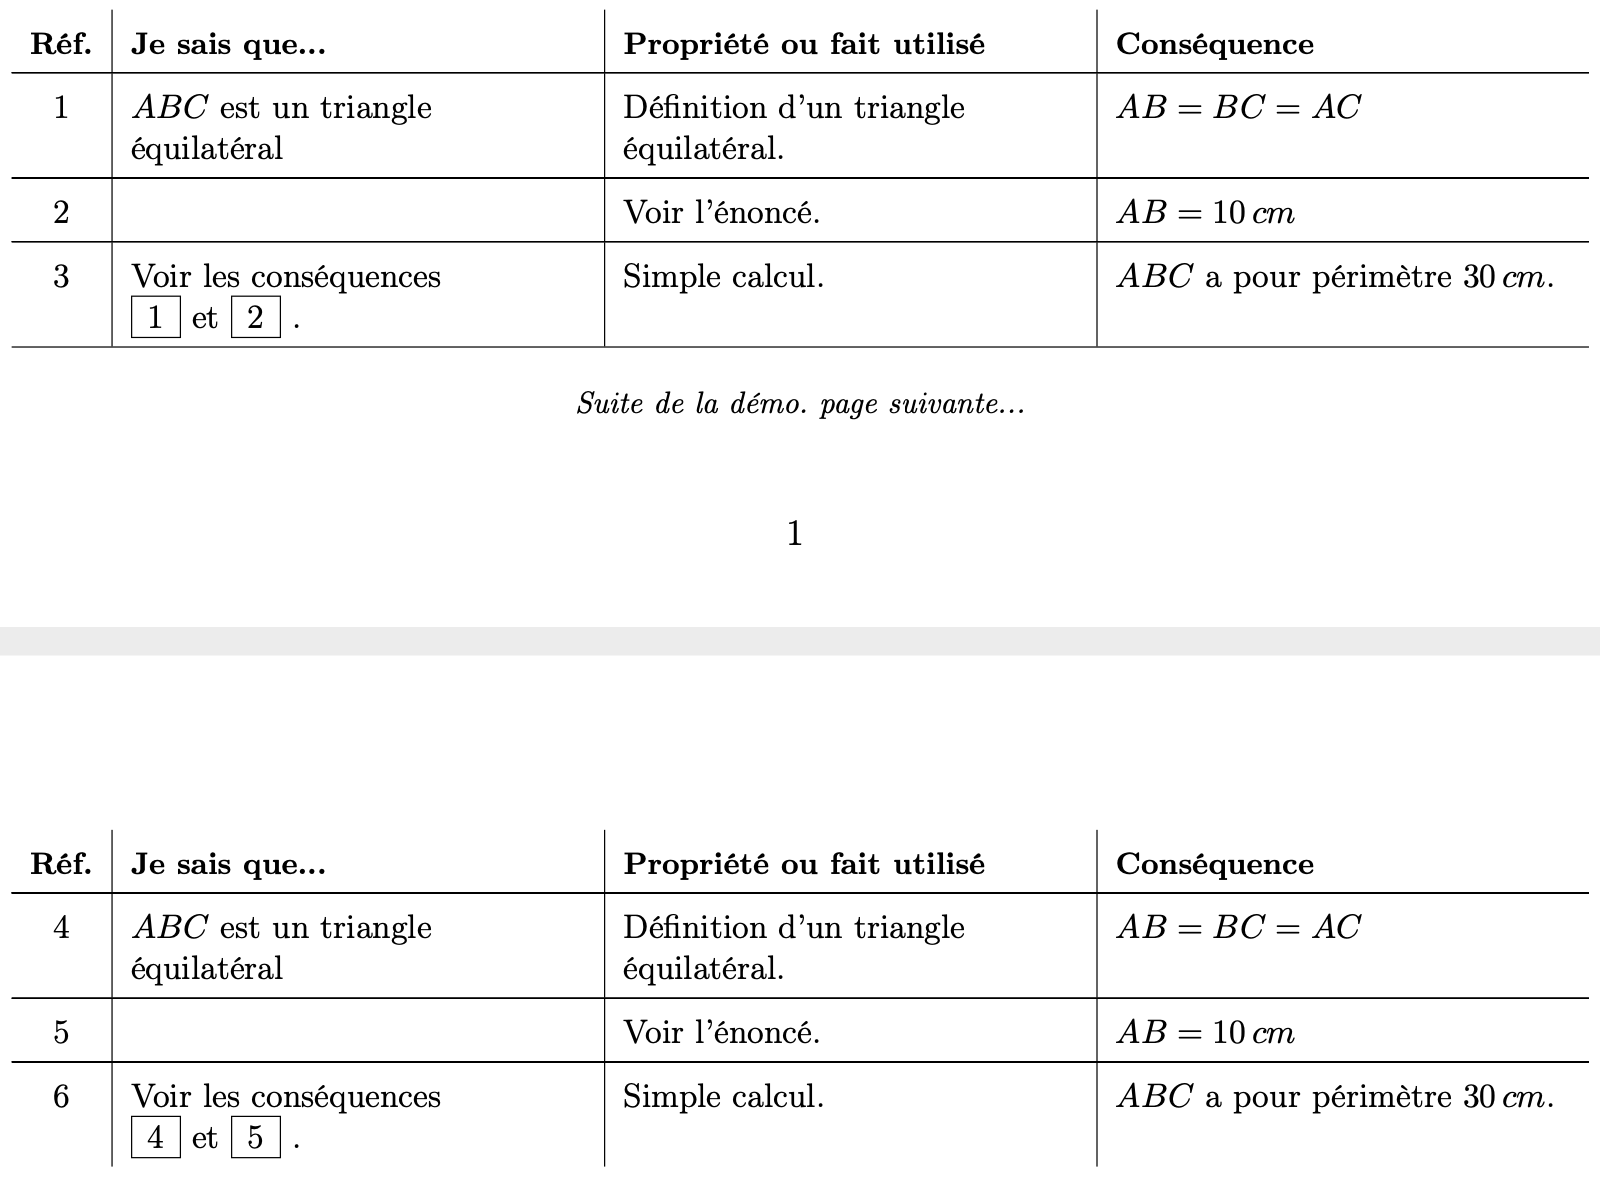
\includegraphics[scale = .5]{images/demo-explained-middleschool-broken[fr].png}}
\end{center}
%\section{Détailler un raisonnement}
\newpage

\section{Historique}

Nous ne donnons ici qu'un très bref historique récent
\footnote{
	On ne va pas au-delà de un an depuis la dernière version.
}
de \verb+tnslog+ à destination de l'utilisateur principalement.
Tous les changements sont disponibles uniquement en anglais dans le dossier \verb+change-log+ : voir le code source de \verb+tnslog+ sur \verb+github+.

\begin{description}
% Changes shown - START

    \medskip
    \item[2020-07-10] Première version \verb+0.0.0-beta+.
% ------------------------ %

% Changes shown - END 
\end{description}


\newpage
\section{Toutes les fiches techniques} \label{techincal-ids}









\subsection{Espace après la négation logique}



\IDope{neg}

\IDope{stdneg} (pour retrouver le symbole par défaut)


\subsection{Différents types de comparaisons \og standard \fg}



\subsubsection{Opérateurs décorés -- Les textes}

\begin{multicols}{4}
% == Technical infos - Texts - START == %

\foreach \k in {textopappli, textopchoice, textopcond, textopcons, textopdef, textophyp, textopid, textopplot, textoptest}{

	\IDmacro[n]{\k}

}

% == Technical infos - Texts - END == %

\end{multicols}

% ---------------------- %


\subsubsection{Opérateurs de comparaison supplémentaires}

% == Technical infos - Operators - START == %

\begin{multicols}{6}
    \foreach \k in {eqdef, eqdef*, eqid, eqid*, eqplot, eqappli, eqchoice, eqcond, eqcons, eqhyp, eqtest}{
        \IDope{\k}

    }
\end{multicols}

\separation

\begin{multicols}{6}
    \foreach \k in {neqid, neqplot, neqappli, neqchoice, neqcond, neqcons, neqhyp, neqtest}{
        \IDope{\k}

    }
\end{multicols}

\separation

\begin{multicols}{6}
    \foreach \k in {lessplot, lessappli, lesschoice, lesscond, lesscons, lesshyp, lesstest}{
        \IDope{\k}

    }
\end{multicols}

\separation

\begin{multicols}{6}
    \foreach \k in {nlessplot, nlessappli, nlesschoice, nlesscond, nlesscons, nlesshyp, nlesstest}{
        \IDope{\k}

    }
\end{multicols}

\separation

\begin{multicols}{6}
    \foreach \k in {leqplot, leqappli, leqchoice, leqcond, leqcons, leqhyp, leqtest}{
        \IDope{\k}

    }
\end{multicols}

\separation

\begin{multicols}{6}
    \foreach \k in {nleqplot, nleqappli, nleqchoice, nleqcond, nleqcons, nleqhyp, nleqtest}{
        \IDope{\k}

    }
\end{multicols}

\separation

\begin{multicols}{6}
    \foreach \k in {gtrplot, gtrappli, gtrchoice, gtrcond, gtrcons, gtrhyp, gtrtest}{
        \IDope{\k}

    }
\end{multicols}

\separation
% == Technical infos - Operators - END == %


\subsection{Équivalences et implications}

\subsubsection{Des symboles logiques supplémentaires}



% == Decorated versions - START == %

\begin{multicols}{4}
    \foreach \k in {iff, iffappli, iffchoice, iffcond, iffcons, iffhyp, ifftest}{
	   \IDope{\k}

    }
\end{multicols}
    
\separation

\begin{multicols}{4}
    \foreach \k in {niff, niffappli, niffchoice, niffcond, niffcons, niffhyp, nifftest}{
	   \IDope{\k}

    }
\end{multicols}
    
\separation

\begin{multicols}{4}
    \foreach \k in {implies, impliesappli, implieschoice, impliescond, impliescons, implieshyp, impliestest}{
	   \IDope{\k}

    }
\end{multicols}
    
\separation

\begin{multicols}{4}
    \foreach \k in {nimplies, nimpliesappli, nimplieschoice, nimpliescond, nimpliescons, nimplieshyp, nimpliestest}{
	   \IDope{\k}

    }
\end{multicols}
    
\separation

\begin{multicols}{4}
    \foreach \k in {liesimp, liesimpappli, liesimpchoice, liesimpcond, liesimpcons, liesimphyp, liesimptest}{
	   \IDope{\k}

    }
\end{multicols}
    
\separation

\begin{multicols}{4}
    \foreach \k in {nliesimp, nliesimpappli, nliesimpchoice, nliesimpcond, nliesimpcons, nliesimphyp, nliesimptest}{
	   \IDope{\k}

    }
\end{multicols}
    
% == Decorated versions - END == %


% ---------------------- %


\subsubsection{Équivalences et implications verticales}



% == Vertical versions - START == %

\begin{multicols}{4}
    \foreach \k in {viff, vimplies, vliesimp}{

	   \IDope{\k}

	   \IDope{n\k}
    }
\end{multicols}

% == Vertical versions - END == %





\subsection{Des versions alternatives du quantificateur existentiel}



\IDmacro[a]{existmulti }{1}

\IDmacro[a]{nexistmulti}{1}

\IDarg{1} une écriture mathématique servant à préciser la portée du quantificateur.


\separation


\IDope{existsone}

\IDope{nexistsone}














\subsection{Détailler un raisonnement simple}



\subsubsection{Détailler un raisonnement simple} 

\IDenv[o]{explain}{1}

\IDoption{} la valeur utilise une syntaxe de type clé-valeur. Voici les différentes clés disponibles.

\begin{enumerate}
	\item \verb+ope+ sert à définir l'opérateur utilisé dans tout l'environnement qui sera rédigé en mode mathématique. 
	      La valeur par défaut est \verb+{=}+ \emph{(et non juste \texttt{=})}.

	\item \verb+style+ sert à définir le style de mise en forme. Voici les différentes valeurs possibles.
	      \begin{enumerate}
	      		\item \prefix{u}, la valeur par défaut, est pour \whyprefix{u}{niversity}.

	      		\item \prefix{ar} est pour \whyprefix{ar}{row}.

	      		\item \prefix{sar} est pour \whyprefix{s}{hort} \whyprefix{ar}{row}.
	      \end{enumerate}

	\item \verb+com+ permet de demander l'alignement ou non des commentaires non étoilés entre eux.
	      \begin{enumerate}
	      		\item \prefix{nal}, la valeur par défaut, est pour \whyprefix{n}{ot} \whyprefix{al}{igned}.

	      		\item \prefix{al} est pour \whyprefix{al}{igned}.

	      \end{enumerate}
\end{enumerate}


\separation


\IDmacro{explnext}{1}{1}  \hfill \mwhyprefix{expl}{ain}

\IDoption{} le symbole à utiliser pour une explication, la valeur par défaut étant celle du symbole de l'environnement \env{explain} où \macro{explnext} est utilisé.

\IDarg{} le texte de l'explication qui peut être vide si aucune explication n'est à afficher.

\medskip

\medskip

\emph{\textbf{ATTENTION !} La macro \macro{explnext} est à utiliser sans argument ni option au tout début du contenu de l'environnement \env{explain} en cas d'utilisation du style \texttt{sar}.}


\separation


\IDmacro{explnext*}{1}{2}

\IDoption{} le symbole à utiliser pour une explication, la valeur par défaut étant celle du symbole de l'environnement \env{explain} où \macro{explnext} est utilisé.

\IDarg{1} le texte de l'explication pour la 1\iere{} ligne.
          Ce texte peut être vide \emph{(voir l'environnement \env{aexplain} pour la raison de ceci)}.

\IDarg{2} le texte de l'explication pour la 2\ieme{} ligne.
          Ce texte peut être vide \emph{(voir l'environnement \env{aexplain} pour la raison de ceci)}.


\separation


\IDmacro[a]{comthis }{1}  \hfill \mwhyprefix{com}{ment}

\IDmacro[a]{comthis*}{1}


\IDarg{} le texte d'un court commentaire.


% ---------------------- %


\subsubsection{Détailler un raisonnement simple -- Mise en forme du texte}

Les macros suivantes sont juste utilisées par l'environnement \env{explain}.


\separation


\IDmacro[n]{expltxtspacein}


\separation


\IDmacro[a]{expltxt}{1}

\IDarg{} le texte de l'explication que l'on veut mettre en forme.


\separation


\IDmacro[a]{expltxtdown}{1}

\IDarg{} le texte de l'explication du haut vers le bas que l'on veut mettre en forme.


\separation


\IDmacro[a]{expltxtup}{1}

\IDarg{} le texte de l'explication du bas vers le haut que l'on veut mettre en forme.


\separation


\IDmacro[a]{expltxtupdown}{2}

\IDarg{1} le texte de l'explication du haut vers le bas que l'on veut mettre en forme.

\IDarg{1} le texte de l'explication du bas vers le haut que l'on veut mettre en forme.


\separation


\IDmacro[a]{explcom}{1}

\IDarg{} le texte d'un court commentaire.








\subsection{Détailler un \og vrai \fg{} raisonnement}



\subsubsection{Détailler un \og vrai \fg{} raisonnement via un tableau}

\IDenv[o]{demoexplain}{4}

\IDkey{start} le début de la numérotation des identifiants des justifications.
              La valeur par défaut est \verb+1+ et la valeur spéciale \verb+last+ permet de reprendre la numérotation là où elle s'était arrêtée le dernier environnement \env{demoexplain} ou \env{demoexplain*} utilisé.

\IDkey{hyps } les hypothèses, au format texte, vérifiées au départ.
              Cet argument peut être vide et ne doit pas rentrer en conflit avec l'option \verb+hyp+.

\IDkey{hyp  } une unique hypothèse, au format texte, vérifiée au départ.
              Cet argument peut être vide et ne doit pas rentrer en conflit avec l'option \verb+hyps+.

\IDkey{ccl  } la conclusion, au format texte, du raisonnement détaillé.
              Cet argument peut être vide.


\separation


\IDenv[o]{demoexplain*}{1}

\IDkey{start} le début de la numérotation des identifiants des justifications.
              La valeur par défaut est \verb+1+ et la valeur spéciale \verb+last+ permet de reprendre la numérotation là où elle s'était arrêtée le dernier environnement \env{demoexplain} ou \env{demoexplain*} utilisé.


\separation


\IDmacro[o]{demostep}{1}

\IDoption{} un texte qui sera utilisé comme label global référençant le numéro d'une justification.


\separation


\IDmacro[a]{explref}{1}  \hfill \mwhyprefix{ref}{erence}

\IDarg{} un numéro de $1$ ou $2$ chiffres qui sera encadré comme le sont les numérotations des indications.


\separation


\IDmacro[a]{explref*}{1}

\IDarg{} un texte correspondant à un label global référençant le numéro d'une justification.


\subsubsection{Détailler un \og vrai \fg{} raisonnement via un tableau - Textes utilisés}

\IDmacro[n]{textdemoID}     \hfill \mwhyprefix{ID}{entifier}

\IDmacro[n]{textdemoKNOWN}

\IDmacro[n]{textdemoPROP}   \hfill \mwhyprefix{PROP}{osition}

\IDmacro[n]{textdemoCONS}   \hfill \mwhyprefix{CONS}{equence}

\extraspace

\IDmacro[n]{textdemoHYPS}   \hfill \prefix{HYPS = HYP-othesis (S-everal ones)} 

\IDmacro[n]{textdemoHYP}    \hfill \prefix{HYP = HYP-othesis (just one)}

\IDmacro[n]{textdemoCCL}    \hfill \prefix{CCL = C-on-CL-usion}

\extraspace

\IDmacro[n]{textdemoNEXTPAGE}




\end{document}
